\clearpage
\section{Database}\label{sec:dati}

\subsection{Schema ER}
\begin{figure}[H]
  \centering
  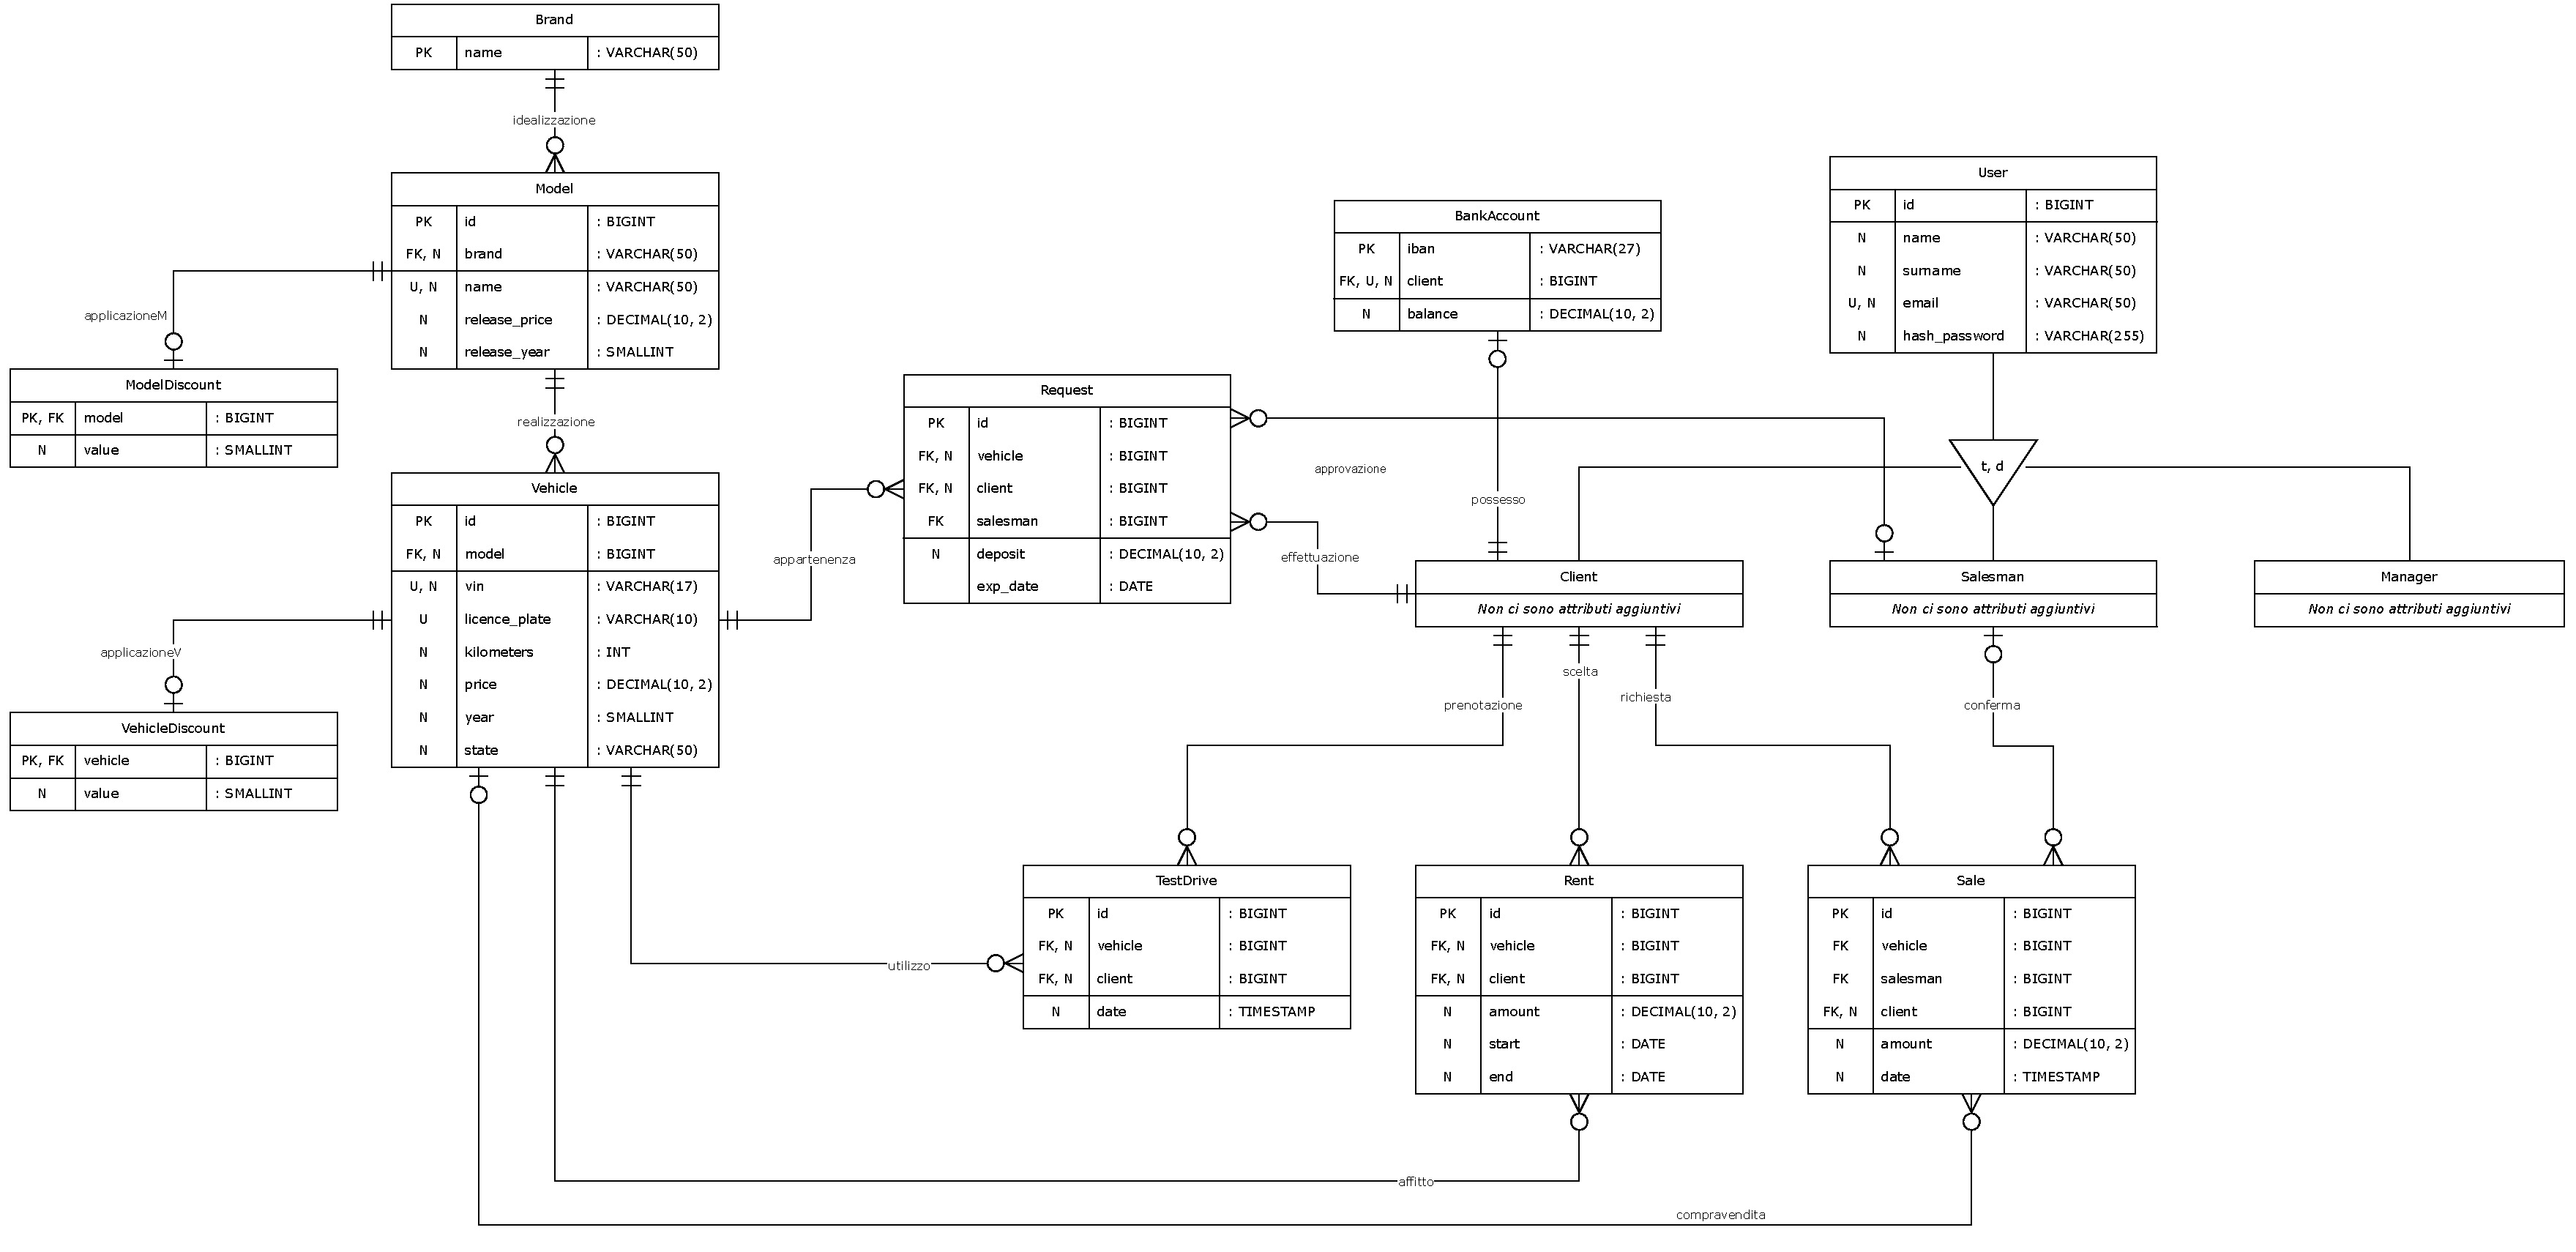
\includegraphics[width=\linewidth,height=.76\textheight,keepaspectratio]{swe-er-original.pdf}
  \caption{Schema entità--relazione di DriveHub, esportato dal diagramma originale dell'autore.}\label{fig:er-drivehub}
\end{figure}
\clearpage
DriveHub conserva catalogo, utenti e operazioni in un database relazionale. La configurazione ordinaria usa PostgreSQL tramite JDBC; la modalità dimostrativa avvia invece H2 in memoria con compatibilità PostgreSQL. Entrambe applicano \code{init.sql}, ma su H2 \code{SqlScriptRunner} omette le istruzioni procedurali specifiche di PostgreSQL, fra cui i trigger. \code{DatabaseBootstrap} registra l'applicazione dello script in \code{drivehub_schema_migrations}, così la migration non viene rieseguita a ogni avvio. Il seed dimostrativo è configurabile ed è attivo per impostazione predefinita. Il conto dei clienti è un saldo simulato nel database: non rappresenta una connessione a un istituto bancario.

La figura~\ref{fig:er-drivehub} riproduce la pagina «schema er» del file originale \texttt{docs/SWE\ ER.drawio}. I simboli alle estremità delle relazioni indicano cardinalità e partecipazione; nelle tabelle, \code{PK}, \code{FK}, \code{U} e \code{N} indicano rispettivamente chiave primaria, chiave esterna, unicità e valore non nullo. Il disegno combina la generalizzazione concettuale degli utenti con gli attributi e le chiavi delle relazioni persistenti.

\noindent\code{Brand} è associata a zero o più \code{Model}, e ciascun modello identifica zero o più \code{Vehicle}. Gli sconti di modello e veicolo sono facoltativi e al più uno per elemento. Un \code{Client} può effettuare più richieste, test drive, noleggi e compravendite. Ogni \code{Request}, \code{TestDrive} e \code{Rent} si riferisce a un cliente e a un veicolo; il \code{Salesman} di una richiesta o vendita è facoltativo. In \code{Sale} è facoltativo anche il veicolo, perché una penale viene registrata senza veicolo. Il medesimo veicolo può comparire in più vendite nel tempo, anche dopo un'acquisizione o una nuova messa in vendita. Il collegamento \code{Client}--\code{BankAccount} indica \code{1..1} sul lato \code{Client} e \code{0..1} sul lato \code{BankAccount}, in accordo con lo schema fisico: ogni conto appartiene a un cliente, mentre un cliente può avere al massimo un conto.

\subsection{Modello relazionale}\label{sec:modello-relazionale}

La traduzione delle relazioni uno-a-molti pone la chiave esterna sul lato «molti». La generalizzazione \code{User} è realizzata con tre tabelle distinte, una per ruolo, che ripetono gli attributi comuni. Lo schema fisico di \code{init.sql} comprende le tredici relazioni seguenti; la vista \code{user} non è una quattordicesima tabella.

\begin{quote}
\ttfamily\small\raggedright
brand(\uline{name})

\smallskip
model(\uline{id}, \dashuline{brand}, name, release\_price, release\_year)\\
\hspace*{2em}\textsc{unique}(name)

\smallskip
model\_discount(\uline{model}$^{\dagger}$, value)

\smallskip
vehicle(\uline{id}, \dashuline{model}, vin, licence\_plate$^{\ast}$,\\
\hspace*{2em}kilometers, price, year, state)\\
\hspace*{2em}\textsc{unique}(vin), \textsc{unique}(licence\_plate)

\smallskip
vehicle\_discount(\uline{vehicle}$^{\dagger}$, value)

\smallskip
client(\uline{id}, name, surname, email, hash\_password)\\
\hspace*{2em}\textsc{unique}(email)

\smallskip
salesman(\uline{id}, name, surname, email, hash\_password)\\
\hspace*{2em}\textsc{unique}(email)

\smallskip
manager(\uline{id}, name, surname, email, hash\_password)\\
\hspace*{2em}\textsc{unique}(email)

\smallskip
bank\_account(\uline{iban}, \dashuline{client}, balance)\\
\hspace*{2em}\textsc{unique}(client)

\smallskip
request(\uline{id}, \dashuline{vehicle}, \dashuline{client},\\
\hspace*{2em}\dashuline{salesman}$^{\ast}$, deposit, exp\_date$^{\ast}$)

\smallskip
test\_drive(\uline{id}, \dashuline{vehicle}, \dashuline{client}, date)

\smallskip
rent(\uline{id}, \dashuline{vehicle}, \dashuline{client}, amount, start, end)

\smallskip
sale(\uline{id}, \dashuline{vehicle}$^{\ast}$, \dashuline{salesman}$^{\ast}$,\\
\hspace*{2em}\dashuline{client}, amount, date)
\end{quote}

\noindent Le chiavi esterne si riferiscono alle seguenti relazioni:
\begin{quote}
\ttfamily\small\raggedright
model.brand $\rightarrow$ brand.name\\
model\_discount.model $\rightarrow$ model.id\\
vehicle.model $\rightarrow$ model.id\\
vehicle\_discount.vehicle $\rightarrow$ vehicle.id\\
bank\_account.client $\rightarrow$ client.id\\
request.vehicle, test\_drive.vehicle, rent.vehicle, sale.vehicle $\rightarrow$ vehicle.id\\
request.client, test\_drive.client, rent.client, sale.client $\rightarrow$ client.id\\
request.salesman, sale.salesman $\rightarrow$ salesman.id
\end{quote}

\begin{samepage}
\noindent\textbf{Legenda della notazione}
\begin{itemize}
\item[] \uline{attributo}: chiave primaria; \dashuline{attributo}: chiave esterna.
\item[] $^{\dagger}$: attributo che è contemporaneamente chiave primaria ed esterna.
\item[] $^{\ast}$: attributo opzionale (\code{NULL} ammesso); gli altri sono obbligatori.
\item[] \textsc{unique}(attributo): vincolo di unicità limitato alla relazione indicata.
\end{itemize}
\end{samepage}

Le date di \code{test_drive} e \code{sale} sono \code{TIMESTAMP}; \code{rent} usa \code{DATE}. Lo schema definisce inoltre \code{CHECK} su prezzi di modelli e veicoli, saldo, importo del noleggio, sconti, stato del veicolo e ordine delle date del noleggio. Non definisce un \code{CHECK} per \code{request.deposit} o \code{sale.amount}: i due campi usano anche valori negativi per distinguere operazioni diverse. Le eccezioni e i limiti di questi vincoli sono spiegati nel paragrafo seguente.

\subsection{Utenti, vincoli e semplificazioni}

Nel diagramma \code{User} raccoglie concettualmente nome, cognome, email e hash della password; \code{Client}, \code{Salesman} e \code{Manager} sono i tre ruoli. La traduzione SQL non crea una tabella \code{user}: replica gli attributi comuni nelle tre tabelle di ruolo e definisce una vista \code{user} mediante \code{UNION ALL}, aggiungendo il campo \code{role}. \code{PostgresUserDao} scrive nella tabella del ruolo e legge dalla vista quando serve una ricerca comune. Gli \code{id} sono generati separatamente nelle tre tabelle e possono quindi coincidere: per identificare un utente fra ruoli occorre considerare anche \code{role}; l'\code{id} mostrato nel supertipo non è una chiave primaria globale della vista.

La registrazione applicativa verifica che l'email non sia già utilizzata e, per un \code{Client}, crea il \code{BankAccount} nella stessa transazione. La relazione uno-a-uno mostrata nel diagramma descrive questo percorso ordinario: nel database \code{UNIQUE(client)} impedisce più conti per lo stesso cliente, ma non obbliga ogni cliente ad averne uno. Per facilitare le prove nella modalità dimostrativa, i trigger sull'email non vengono installati su H2. Su PostgreSQL \code{init.sql} definisce invece la funzione \code{check_user_email_disjoint} e tre trigger, ma il loro confronto esclude righe con lo stesso \code{id} numerico anche se provengono da tabelle diverse. Gli ID dei ruoli sono indipendenti, quindi i trigger non assicurano l'unicità trasversale in tutti i casi. \code{UNIQUE(email)} vale all'interno di ciascuna tabella; il normale percorso di registrazione esegue anche una ricerca preventiva nella vista \code{user}.

Le regole espresse nello schema includono, fra le altre, \code{UNIQUE} su VIN e targa, saldo non negativo, sconti fra 0 e 50, stato del veicolo limitato a \code{WAITING}, \code{SALE}, \code{RENT}, \code{BLOCKED} e \code{SOLD}, e fine del noleggio non precedente all'inizio. Altre condizioni restano applicative: non esiste un vincolo SQL che impedisca la sovrapposizione temporale di due \code{Rent} o renda unico lo slot di \code{TestDrive}. Il segno di \code{Request.deposit} distingue l'acconto d'acquisto dalla stima di cessione; il segno di \code{Sale.amount} distingue la vendita dall'esborso per un'auto acquisita. Una penale è una \code{Sale} con \code{vehicle} e \code{salesman} nulli. Lo schema consente queste rappresentazioni, ma non contiene \code{CHECK} che ne garantiscano tutte le combinazioni ammissibili.
